\tikzsetfigurename{module4_2_14_ingeschrevenCirkel}
	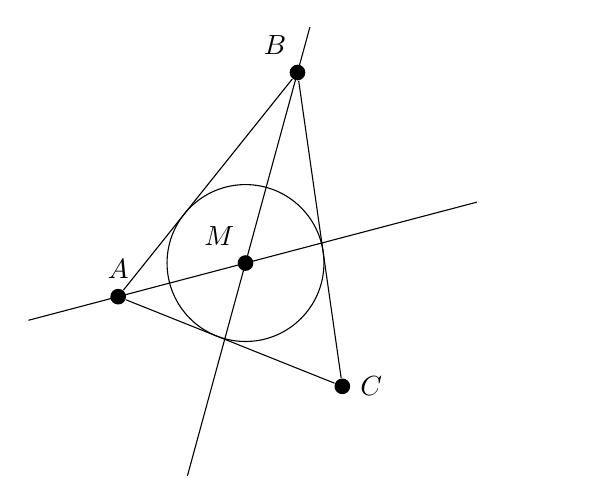
\begin{tikzpicture}
\begin{axis}[xmin=-5, xmax=7, ymin=-5, ymax=5,
axis lines = middle,xlabel=\empty,ylabel=\empty, axis equal, axis line style={draw=none},
xtick=\empty, ytick=\empty,
tick style={draw=none},
domain=-5:5,
samples=101,
smooth,
no markers]
\draw (axis cs: -0.16, -0.25) circle [radius=1.75];
%	\addplot[red,mark=*] coordinates {(2,3)};
\node[label={100:{$M$}},circle,fill,inner sep=2pt] at (axis cs:-0.16,-0.25) {};
\node[label={90:{$A$}},circle,fill,inner sep=2pt] (A) at (axis cs:-3,-1) {};
\node[label={100:{$B$}},circle,fill,inner sep=2pt] (B) at (axis cs:1,4) {};
\node[label={0:{$C$}},circle,fill,inner sep=2pt] (C) at (axis cs:2,-3) {};
%	\node[label={270:{$A$}},circle,fill,inner sep=2pt] at (axis cs:2,1) {};

\draw[-](A)--(B);
\draw[-](B)--(C);
\draw[-](C)--(A);

\addplot[black] {14.11/53.556*x-11.198/53.556};
\addplot[black] {80.177/21.881*x+7.347/21.881};

\end{axis}

%	\draw[->] (-5,0)--(5,0) node[anchor=south,left,yshift=0.2cm]{$x$};
%	\draw[->] (0,-4)--(0,6) node[anchor=south,left]{$y$};
%	
%	\tkzDefPoint(0,0){S}
%	\tkzDefPoint(1,0){x1}
%	\tkzDefPoint(0,1){y1}
%	
%	\tkzDefPoint(-3,0){A1}
%	\tkzDefPoint(0,-1){A2}
%	
%	\tkzDefPoint(-3,-1){A}
%	
%	\tkzDefPoint(1,0){B1}
%	\tkzDefPoint(0,4){B2}
%	
%	\tkzDefPoint(1,4){B}
%	
%	\tkzDefPoint(2,0){C1}
%	\tkzDefPoint(0,-3){C2}
%	
%	\tkzDefPoint(2,-3){C}
%	
%	\tkzLabelPoint[below,xshift=-0.1cm](S){$0$}
%	%	\tkzLabelPoint[right,yshift=-0.3cm](S){$O$}
%	
%	\tkzLabelPoint[below](x1){$1$}
%	\tkzLabelPoint[left](y1){$1$}
%	
%	\tkzLabelPoint[left,yshift=0.2cm](A){$A$}
%	\tkzLabelPoint[right,yshift=0.2cm](B){$B$}
%	\tkzLabelPoint[right,yshift=0.2cm](C){$C$}
%	
%	\tkzLabelPoint[above](A1){$-3$}
%	\tkzLabelPoint[right](A2){$-1$}
%	
%	%	\tkzLabelPoint[below](B1){$-1$}
%	\tkzLabelPoint[left](B2){$4$}
%	
%	\tkzLabelPoint[above](C1){$2$}
%	\tkzLabelPoint[left](C2){$-3$}	
%	
%	\tkzDrawSegment[black!60!black,dotted](A1,A)
%	\tkzDrawSegment[black!60!black,dotted](A2,A)
%	\tkzDrawSegment[black!60!black,dotted](B1,B)
%	\tkzDrawSegment[black!60!black,dotted](B2,B)
%	\tkzDrawSegment[black!60!black,dotted](C1,C)
%	\tkzDrawSegment[black!60!black,dotted](C2,C)
%	
%	\tkzDrawSegment[black!60!black](A,C)
%	\tkzDrawSegment[black!60!black](A,B)
%	\tkzDrawSegment[black!60!black](B,C)
%	
%	\foreach \n in {S,x1,y1,A1,A2,A,B1,B2,B,C1,C2,C}
%	\node at (\n)[circle,fill,inner sep=1.5pt]{};

\end{tikzpicture}